\section{Architecture du projet}


Réfléchir à ce projet en modules était important, le projet nécessite d'implémenter beaucoup d'éléments différents et les implémenter tous au sein d'un seul fichier n'était pas une idée réaliste du tout. Il a fallu réfléchir à comment segmenter le travail pour éviter les bugs qui freinent l'ensemble de l'avancée.


\subsection{Découpage en modules}

En se basant sur nos imports notre projet peut être découpé en 4 couches. On a une première couche \texttt{World} qui comprend les fichiers \textit{world.ts et puzzle.ts}, ces fichiers définissent tous les types nécessaires (\texttt{Puzzle, Cell, Robot et World}) ainsi que les objectifs présents sur le monde. Ces deux fichiers constituent le socle du projet définissant l'ensemble des outils dont on a besoin pour réaliser le projet. 
\bigskip
Ensuite on a une autre couche qui se concentre sur \texttt{la pile de jeu}. L'un des aspects les plus importants du projet est la mise en place d'une \texttt{pile de jeu} comprenant des instructions et des fonctions ainsi que \texttt{la mise en relation} de ces dites instructions et du monde. Cette couche est donc multifonctionnelle, elle gère aussi bien les actions du robot que les conditions et les réponses de ces dites actions par rapport au monde. 

\begin{figure}[H]
    \centering
    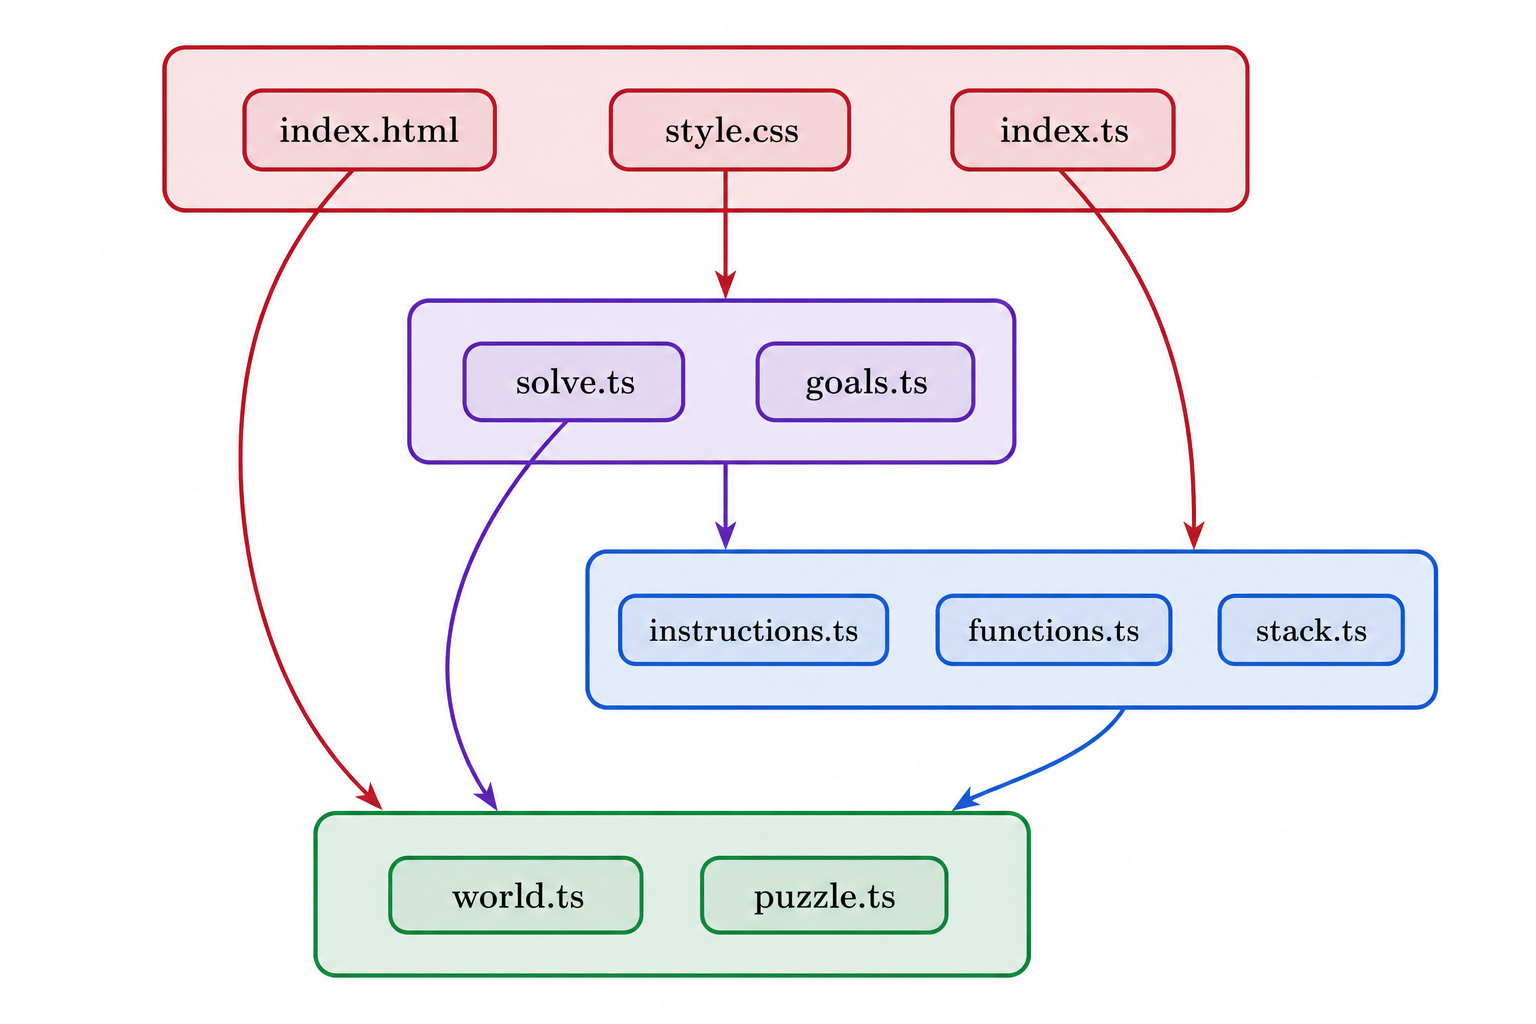
\includegraphics[width=0.8\textwidth]{images/image_arch.png}
    \caption{Graphe des dépendances}
    \label{fig:architecture}
\end{figure}

Enfin vient une couche composée de deux fichiers \textit{solve.ts et goals.ts} dans la Figure~\ref{fig:architecture}. cette couche gère la conception d'une solution à un puzzle donné.
 le fichier \textit{goals.ts} s'occupe de faire le décompte des objectifs pendant que \textit{solve.ts} gère la résolution du puzzle. Ce dernier vérifie qu'une pile donnée résout bien le puzzle. 
 Ainsi cette couche doit faire appel aux deux autres couches car elle demande \texttt{la conception d'une pile pour résoudre un monde}.

La dernière couche s'occupe de l'affichage, on y retrouve les fichiers \textit{index.ts, index.html et style.css}. Cela met en lumière \textit{la multidépendance} de toutes les couches fonctionnelles.

\subsection{Pile d'exécution}

Une particularité de notre architecture est que les fichiers établissant notre pile d'appel \textit{instructions.ts, function.ts et stack.ts} s'incluent mutuellement, ce qui fait des inclusions circulaires. 
Toutefois la particularité fonctionnelle du projet permet d'importer uniquement les fonctions dont on a besoin se mettant ainsi à l'abri des inclusions circulaires en tant que tel.

\begin{figure}[H]
    \centering
    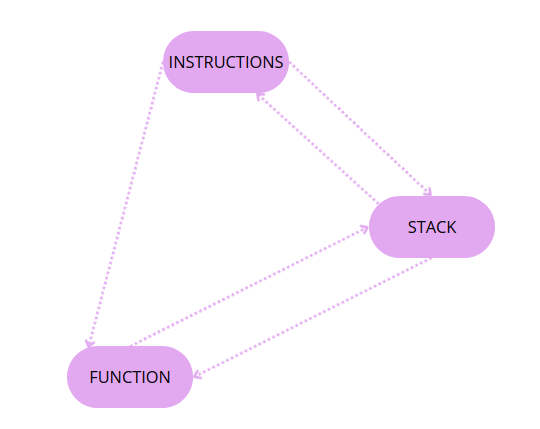
\includegraphics[width=0.5\textwidth]{images/img1.png}
    \caption{Dépendances circulaires au sein du module pile}
    \label{fig:architecture2}
\end{figure}

